\chapter{Demonstrating the Tool}\label{chap:case_study}
This chapter will demonstrate how to use the Xpand framework together with the DPF metamodel and its Eclipse integration. We will generate code for the Play~\cite{playframework} web framework based on a simple DSML. Generating code for a web framework is an excellent use case, because of the similar traits from one application to another. 
% If one defines two web applications in the same framework, they will most likely share the same structure. This makes web applications a popular domain for MDE and code generation~\cite{Vis08}~\cite{uwe4jsf}. 

\section{Components/Packages}
\begin{description}
  \item[\codeText{no.hib.dpf.codegen.examples.dpfplay}] \hfill \\
  Contains the generator implementation.
  \item[\codeText{no.hib.dpf.codegen.examples.dpfplay.ui}] \hfill \\
  This plug-in contains the Eclipse integration for the generator.
\end{description}

The component name chosen is \codeText{codegen} like the DPF Xpand metamodel. The sub component is called examples, as a common subcomponent for all code generation related example projects. The name chosen for the project is "dpfplay".
\begin{quote}
  \emph{NOTE: The plug-ins are part of the reference example project. This chapter will not explain the Eclipse integration found in the \codeText{no.hib.dpf.codegen.examples.dpfplay.ui} plug-in.}
\end{quote}

\section{Choosing a Framework}
The following is a short evaluation of the candidates chosen for this tool demonstration. The criterias used was simple;
a modern framework with as little configuration and boilerplate\footnote{Boilerplate code is a term for code which appears in many places with little to none alterations.} code as possible.  Most popular frameworks today is based on the \emph{Model View Controller (MVC)} pattern, which give them similar properties. If one defines two web applications in the same framework, they will most likely share the same structure. This makes web applications a popular domain for MDE and code generation~\cite{Vis08}~\cite{uwe4jsf}. 

The model part of an MVC framework is usually the most generic and simple to generate code for. \emph{Controllers} and \emph{View} vary a lot more in how they function.  

After a short evaluation the Play Framework was chosen. In addition to fitting the criterias, it is made for Java (and Scala) which was ideal considering the time left in the project. As we will discover, Play enables us to get results with very little code.

\subsection{Lift}
Lift~\cite{liftweb} is a web framework based on the Scala programming language, which focuses on security, scalability and ease of use. The framework tries to fill the same need as other web frameworks such as Ruby-on-Rails and Spring, but tries to improve on the shortcomings other frameworks exhibits. Lift follows the MVC pattern to enforce separation of concern; unlike JSP, Lift does not allow code in the templates. The framework also benefits from Scala's Actor model which provides concurrency in a safe and robust manner. 

\subsection{Django}
Django~\cite{django} is another web framework based on the MVC paradigm which uses the Python programming language. Its focus is to hide the boilerplate code and focus on the functionality. 
Among the wide range of features you find Object-Relational Mapping (ORM), caching framework, template engine, a standalone web-server and automatically generated CRUD interface for your model classes. 

\subsection{Grails}
Grails~\cite{grails} uses the Groovy programming language which is a dynamic language running on the JVM. As with Django and Lift, Grails uses
the MVC pattern. Under the hood it uses a lot of the functionality inside Spring, but stays clear of any XML configuration.

\subsection{Play Framework}
The Play Framework~\cite{playframework} is a MVC web framework for Java and Scala. It aims to be a more effective alternative to other Java frameworks like Spring and Java EE. Play comes with its own runtime that loads code changes directly into the JVM, and removes the need to restart the application server each time a change is made. Another notable feature is the template engine, which uses Groovy as expression language. The result is a concise syntax with less boilerplate code.

\section{Problem Description}
Creating a working example for the code generation tool is needed to demonstrate how it works. The process of creating a generator project is simple, yet it demands some hand coding to create the templates, which are the most important part. Any UI integration of the generator will need to be hand coded in the same manner as any other Eclipse plug-in.

Through this chapter we will demonstrate a simple code generator, which generates simple Java model classes for the Play framework using a simple DSML. We will utilize Play's built-in modules to provide a CRUD (Create, Read, Update, Delete) interface using our generated classes. 

This chapter acts as a tutorial on how to use the code generation tool. The code for this example project can be found at \url{http://dpf.hib.no/downloads/}. It contains a more elaborate example with Eclipse integration for the generator. 

This example project was developed using Eclipse Indigo (modelling tools bundle) with Xpand and the DPF Xpand metamodel installed. The version of Play framework used is 1.2.4.

% The project contains some UI integration with Eclipse so that we get a sense on how to integrate the generator as part of the UI workflow, and not running the workflow file directly through the Modeling Workflow Engine (MWE, see~\ref{subsub:workflow}). The tool will use DSML which is hard coded as the typing of an editor. This editor can create model classes for Play! based on the hard coded typing. Generating code happens through user interaction, where the instance model gets passed to the generator for processing.

\section{Creating the Generator}
\subsection{What to Generate}
As stated in the previous section, we want to generate simple model classes for a Play project. The example is very simple, and will not entail the generation of any behaviour oriented code. We will handle multiplicity constraints to give an example on how to use them in their current state. In section~\ref{sec:create_generator} we briefly discuss the creation of a code generator and what is needed for creating one; mainly a sample input and output to clearly define the generator's requirements. The templates in the generator can be regarded as transformation rules, and it is thus necessary to see what you want to transform and what it should result in.

The first thing we need to do is define a DSML for our problem. This step is not necessarily a part of the code generation activity, as the language might be pre-defined.
% \newpage

\begin{figure}[h]
  \centering
  \centerline{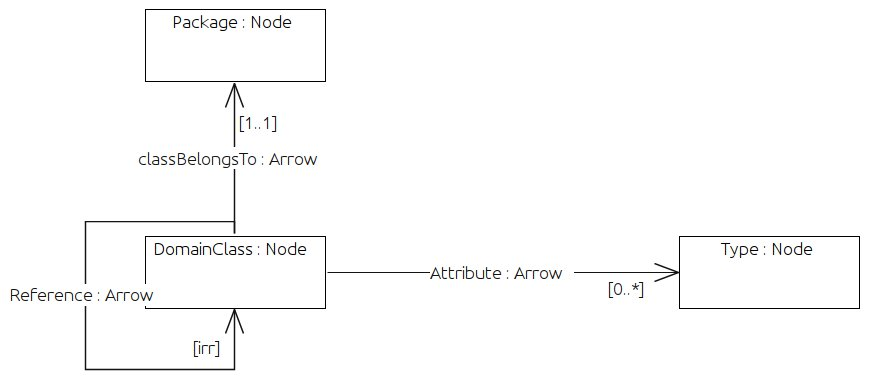
\includegraphics[scale=0.5]{images/web_dsml.jpeg}}
  \caption[DSML for dpfplay]{Figure depicts a simple DSML for creating domain classes.}
  \label{fig:web_dsml}
\end{figure}

Lets go through the DSML step by step:
\begin{enumerate}
  \item We define three \codeText{Nodes} which have the type names \codeText{DomainClass}, \codeText{Type} and \codeText{Package}.
  \item A \codeText{DomainClass} may have a \emph{reference} to one or more \codeText{DomainClasses}.
  \item A \codeText{DomainClass} can not reference itself. This is enforced by the irreflexive \codeText{[irr]} constraint.
  \item A \codeText{DomainClass} has exactly one \codeText{Package} (\codeText{[1..1]} multiplicity constraint).
  \item A \codeText{DomainClass} can have zero or more \codeText{Types} associated.
\end{enumerate}

In short, this DSML enables us to create \codeText{DomainClass} nodes that belongs to a \codeText{Package}. The \codeText{DomainClass} may or may not have any attributes or other \codeText{DomainClasses} associated with it.

To properly understand how to create our generator, we need to create a sample input model:
\begin{figure}[h]
  \centering
  \centerline{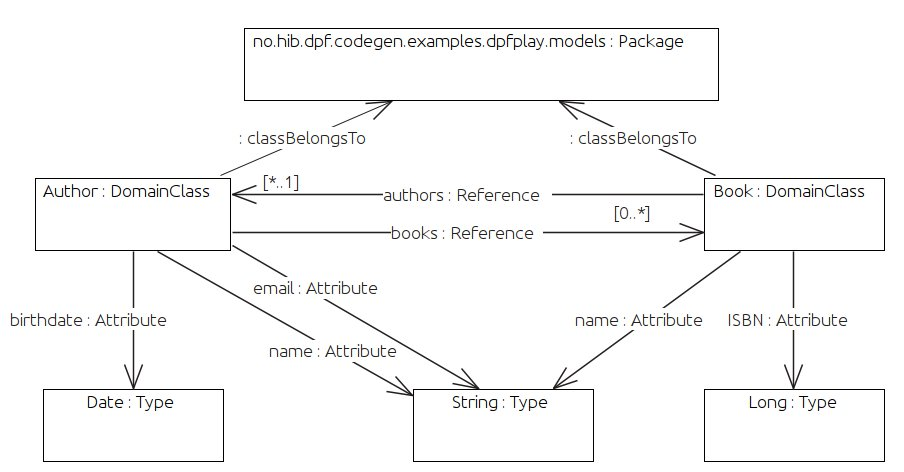
\includegraphics[scale=0.5]{images/dsml_instance.jpeg}}
  \caption[Sample instance model for dpfplay]{An instance model for the DSML (\ref{fig:web_dsml}).}
  \label{fig:web_instance}
\end{figure}

The instance model in figure~\ref{fig:web_instance} shows an example with nodes \codeText{Author} and \codeText{Book} which both are typed by \codeText{DomainClass}. Each node has a few attributes shown by the arrows typed by \codeText{Attribute}. There are also a zero-to-many relation between \codeText{Author} and \codeText{Book} (an author can have zero or more books), as well as a one-to-many relation from \codeText{Book} to \codeText{Author} (one book can have many authors).

Now that we have a sample input defined, we can define what we want to achieve with the generator. This example will create very simple model classes which forms the foundation in a Play web application. 

\lstset{language=Java,caption=Listing shows a preliminary draft of the code we want to generate.,label=list:gencode,captionpos=b}
\begin{table}[hp]
  \centering
\begin{lstlisting}[showstringspaces=false]
Author.java

package no.hib.dpf.codegen.examples.dpfplay.model;

import java.util.Date;
import java.util.ArrayList;

public class Author {
  public String name;
  public String email;
  public Date birthdate;
  public ArrayList<Book> books;

  public Author(String name, String email, Date birthdate, ArrayList<Book> books) {
    this.name = name;
    this.email = email;
    this.birthdate = birthdate;
    this.books = books;
  }
}

Book.java

package no.hib.dpf.codegen.examples.dpfplay.model;

import java.util.ArrayList;

public class Book {
  public String name;
  public String isbn;
  public ArrayList<Author> authors;

  public Book(String name, String email, ArrayList<Author> authors) {
    this.name = name;
    this.isbn = isbn;
    this.authors = authors;
  }
}
\end{lstlisting}
\end{table}

Listing~\ref{list:gencode} shows a draft of how we would like the code to look after code generation. The seasoned reader might see that we have defined our data fields as \emph{public}, rather than \emph{private}. This is an example of the convenience Play provides through its own runtime; all public fields will have getters and setters generated. Model classes in Play will typically also contain Java Persistence API (JPA) annotations for the persistence of the models. These will be added at a later point.

Now that we have defined our DSML, instance model and output sample, we can start thinking about creating a generator project and define our templates.

\subsection{Creating a Generator Project}
When selecting the \emph{New} wizard in Eclipse, we find a new entry under the DPF category, \emph{DPF Generator Project}. This is part of the functionality we defined in the \codeText{no.hib.dpf.codegen.xpand.ui} plug-in.

\begin{itemize}
  \item \emph{Select DPF Generator Project as figure~\ref{fig:codegen_wizard1} shows.}
\end{itemize}

\begin{figure}[h]
  \centering
  \centerline{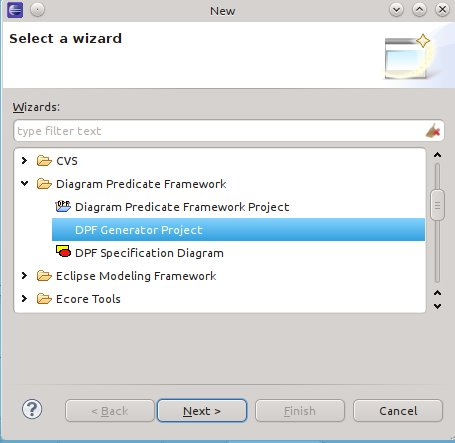
\includegraphics[scale=0.53]{images/codegen_wizard1.jpeg}}
  \caption[Eclipse wizard]{Eclipse \emph{new} wizard showing the DPF category with DPF Generator Project.}
  \label{fig:codegen_wizard1}
\end{figure}

Figure~\ref{fig:codegen_wizard2} shows the DPF Generator Wizard. As shown, there are two fields in the wizard. The project name is obligatory while the location of the DSML is optional. As discussed in section~\ref{subsec:editor_support}, the DSML is needed to enable the editor support. Even though a DSML is not defined for the project you create, one can define the location where it is supposed to be. The DSML will then load upon creation. One can also use the location of DSMLs in other projects in the workspace. We will leave the metamodel location blank for now, as we wish specify it later.

\begin{figure}[h!]
  \centering
  \centerline{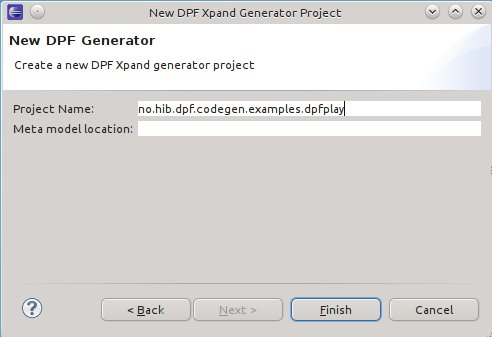
\includegraphics[scale=0.7]{images/codegen_wizard2.jpeg}}
  \caption[DPF Generator wizard]{Figure shows the DPF Generator Wizard.}
  \label{fig:codegen_wizard2}
\end{figure}

\begin{itemize}
  \item \emph{Set project name to \codeText{no.hib.dpf.codegen.examples.dpfplay}}.
  \item \emph{Leave metamodel location blank and press "Finish"}.
\end{itemize}

We have now a ready to use project structure (see~\ref{subsec:project_structure}). As the DSML location has not been defined, the generated template stub will show an error as the \codeText{dpf} namespace is not found.

Before proceeding, we want to define the DSML and instance model using the DPF Editor, so that we can get editor support in the later steps.

\begin{itemize}
  \item \emph{Create a new folder \textbf{models} in our project.}
  \item \emph{Inside the \textbf{models} folder, create a new DPF specification with the name "metamodel".}
%   \item \emph{The \textbf{models} folder should now contain a "metamodel.dpf" and a "metamodel.dpf.xmi".}
  \item \emph{Open the specification and define the DSML in figure~\ref{fig:web_dsml}.}
  \item \emph{Create another DPF specification with the name "author" within the \textbf{model} folder. Use "metamodel.dpf.xmi" as the typing for the specification.}
  \item \emph{Open the specifcation and define it using our model from figure~\ref{fig:web_instance}.}
\end{itemize}

\subsection{Defining the Workflow}
With the project structure a workflow is generated, it contains almost everything that is needed to run it. The generated workflow should look like so:

\lstset{language=XML,caption=The generated workflow file in a DPF Generator Project,label=list:codegenworkflow,captionpos=b}
\begin{table}[h]
  \centering  
  \begin{lstlisting}[showstringspaces=false]
<?xml version="1.0" encoding="UTF-8" standalone="no"?>
<workflow>
  <!-- workflow properties -->
  <property name="dpf_model" value=""/>
  <property name="dpf_metamodel" value=""/>

  <property name="src-gen" value="src-gen"/>

  <!-- set up EMF, only needed when using URI's -->	
  <bean class="org.eclipse.emf.mwe.utils.StandaloneSetup">
      <platformUri value=".."/>
  </bean>
	
  <!-- instantiate metamodel-->
  <bean class="no.hib.dpf.codegen.xpand.metamodel.DpfMetamodel" id="mm_dpf"/>
	
  <!-- DPF component -->
  <component class="no.hib.dpf.codegen.xpand.metamodel.workflow.DpfReader">
      <dpfMetaModel value="${dpf_metamodel}"/>
      <dpfModel value="${dpf_model}"/>
      <metaModel idRef="mm_dpf"/>
      <modelSlot value="dpf"/>
  </component>
	
  <!--  generate code -->
  <component class="org.eclipse.xpand2.Generator">
      <metaModel idRef="mm_dpf"/>
      <expand value="template::templ::main FOR dpf"/>
      <outlet path="${src-gen}">
	  <postprocessor class="org.eclipse.xpand2.output.JavaBeautifier"/>
      </outlet>
  </component>
</workflow>
  \end{lstlisting}
\end{table}

\newpage

As listing~\ref{list:codegenworkflow} shows, we get a workflow file with the DPF Reader component inserted (see~\ref{subsub:workflow} for an explanation of a workflow). The only attributes which must be set is the location for a DSML and an instance model.

\begin{itemize}
  \item \emph{Insert the DSML's path \codeText{models/metamodel.dpf.xmi} into the\newline \codeText{dpf\_metamodel} property's value attribute.}
  \item \emph{Insert the instance model's path \codeText{models/author.dpf.xmi} into the\newline \codeText{dpf\_model} property's value attribute.}
  \item \emph{Save the file.}
\end{itemize}
Defining the instance model at this moment, does not affect anything as it is only used when running the generator. The definition of the DSML on the other hand is more interesting; every time a resource gets changed in the project, we scan it and try to retrieve a valid path to a DSML. The first check is to see if a workflow file is defined. If so, it will look for the \codeText{dpf\_metamodel} attribute and see if a value is defined. If a value is defined, it will mirror the path in the \emph{no.hib.dpf.codegen.xpand.ui.prefs} file and load the specifcation for use in the DPF Xpand metamodel. If no such value is found in the attribute, the tool will try to find a path in the \emph{no.hib.dpf.codegen.xpand.ui.prefs} file. If this fails as well, no metamodel will be loaded for the project. This solution is admittely not the most optimal, as it will not work with more than one DSML per project (in its current state).

\subsection{Defining the Template}
Now that we have defined a DSML in the workflow file, we get editor support. We have defined our input model as well, and created a draft of our output. We will now define a template for creating model classes and use Xtend and Java extensions where it is needed.

\begin{quote}
  \emph{NOTE: When creating/reading templates in Xpand, make sure that the font encoding is set to UTF-8 or another encoding which support \emph{guillemets} (« and »).}
\end{quote}

\subsubsection{Basic Xpand Concepts}
\begin{itemize}
  \item \emph{Open the templ.xpt file.}
\end{itemize}
\flushleft The only content of the file is:
% \lstset{title=,caption=} %DO NOT CHANGE OR SET LIST CAPTION BEHIND THIS WITHOUT RESETTING
\begin{plainlisting}
«IMPORT dpf»

«DEFINE main FOR dpf::Specification»

«ENDDEFINE»
\end{plainlisting}{}
A \codeText{DEFINE} block for a \codeText{Specification} type is required to start with, as it is the assumed input object for the generator. \codeText{DEFINE} statements are also called \emph{definitions} or \emph{templates}. The \codeText{DEFINE} statements are the building blocks of the template files; each statement can invoke other \codeText{DEFINE} statements and so on. 

In our example template, the \codeText{main} block engulfs all of the other \codeText{DEFINE} blocks. The \codeText{main} block is invoked through the workflow engine using \codeText{<expand~value="template::templ::main~FOR dpf"/>}. \codeText{dpf} is the \emph{model slot} defined in the DPF Reader (see~\ref{subsec:reader_workflow}). The \codeText{Specification} object that represents a DPF model has a hierarchy which is reflected in the templates we create. 

The next step in our template is to create a \codeText{DEFINE} statement for a graph.
\begin{quote}
  \emph{NOTE: Guillemets are created using \emph{Ctrl+<} for « and \emph{Ctrl+Shift+<} for ».}
\end{quote}
\begin{itemize}
  \item \emph{Add the following listing to templ.xpt:}
  \begin{plainlisting}
«DEFINE graph FOR dpf::Graph»

«ENDDEFINE»
  \end{plainlisting}
\end{itemize}
To invoke the \codeText{graph} block from \codeText{main}, we need an \codeText{EXPAND} statement. The \codeText{EXPAND} statement is used for invoking other \codeText{DEFINE} blocks.
\begin{itemize}
  \item \emph{Inside the \codeText{main} block, add:}
  \begin{plainlisting}
«EXPAND graph FOR this.graph»
  \end{plainlisting}
\end{itemize}
The \codeText{EXPAND} statement expands the \codeText{graph} block with the \codeText{Specification} object's internal \codeText{graph} object. The \codeText{this} handle refers to the object which the \codeText{DEFINE} block pertains to. 

Our DSML defines the concept \codeText{DomainClass} which represents a model class for use in a Play web application. The next step in our template is to iterate over every \codeText{DomainClass} which is defined in the instance model.
\begin{itemize}
  \item \emph{Create a new \codeText{DEFINE} statement:}
  \begin{plainlisting}
«DEFINE domainclasses FOR dpf::DomainClass»

«ENDDEFINE»
  \end{plainlisting}
  \item \emph{Add the following line to the \codeText{graph} \codeText{DEFINE} block:}
  \begin{plainlisting}
«EXPAND domainclasses FOREACH this.getDomainClasses()»
  \end{plainlisting}
\end{itemize}
We start to see how the DPF Xpand metamodel lets us express the concepts of our DSML rather than the DPF Ecore model (see section~\ref{sec:problem_description} for an example). The \codeText{getDomainClasses()} method is a custom convenience method defined in the DPF Xpand metamodel's \codeText{GraphType}. Using this method we iterate over every \codeText{DomainClass} instead of its type node, \codeText{Node}. An important observation is that we use \codeText{FOREACH} when we want to invoke a \codeText{DEFINE} statement for each element in a collection.

In Java, a class is defined in its own file. This means we need to create a Java class file for each \codeText{DomainClass} type in our instance model. This is achieved using the \codeText{FILE} statement.
\begin{itemize}
  \item \emph{Inside the \codeText{domainclasses} block, add:}
\lstset{label=list:gencode,captionpos=b}
  \begin{plainlisting}
«FILE this.name.toFirstUpper() + ".java"»
«ENDFILE»
  \end{plainlisting}
\end{itemize}
The \codeText{FILE} statement creates a file with a name as argument. The example shows that we retrieve the \codeText{name} of the current \codeText{DomainClass} using \codeText{this}. We also take advantage of the built-in string operation \codeText{toFirstUpper()} that returns the name with the first letter as uppercase.

\begin{itemize}
  \item \emph{Run the MWE workflow by right-clicking the workflow file and selecting "Run As -> MWE Workflow".}
\end{itemize}
We should now see two empty files called "Author.java" and "Book.java" in our \codeText{src-gen} folder.

The basic constructs of Xpand are now familiar and we can start defining the content of the files we generate. From within the \codeText{FILE} block we can insert the first statements.

\subsubsection{Creating an Extension}
\begin{itemize}
  \item \emph{Inside the \codeText{FILE} block, add:}
  \begin{plainlisting}
package «this.getAClassBelongsTos().get(0).target.name»;
  \end{plainlisting}
  \item \emph{Run the workflow.}
\end{itemize}
When executing the workflow, we generate two files which only contains a package declaration in the \codeText{src-gen} folder. Although the statement looks a bit messy, the semantics are easy to grasp. From the current \codeText{DomainClass} type, we retrieve all the outgoing \codeText{classBelongsTo} arrows. The DPF Xpand metamodel defines every getter for an outgoing arrow as a collection for consistency reasons throughout the tool, despite the use of a \codeText{[1..1]} multiplicity constraint on the particular arrow. When we have retrieved the arrow, we call the target attribute, which retrieves the node that the arrow points to, and lastly we fetch the target node's name. We observe that Eclipse displays an error icon on our generated files, and tells us that the files are in the wrong package. This happens because we have told the generator to output everything to the \codeText{src-gen} directory. In our metamodel we have specified that each model class can have its own package which means we do not want to hardcode the package path. Fortunately we can delimit the \codeText{FILE} statement's name argument with a slash, thus defining the output file's path.

Creating a valid path for the \codeText{FILE} statement is an example on where you can use extensions, rather than perform program logic within the template. Replacing all "." with a "/" is done using a single line of code, but it will look tidier with a descriptive method name.
\begin{itemize}
  \item \emph{Create a new package called \codeText{extensions}.}
  \item \emph{Create a new file in the \codeText{extensions} package called \textbf{dpfplay.ext}.}
  \item \emph{Insert the following code:}
  \begin{plainlisting}
import dpf;
getPackage(DomainClass d):
    d.getAClassBelongsTos().get(0).target.name.replaceAll("\\.", "/") + "/";
  \end{plainlisting}
  \item \emph{Insert the following right below the \codeText{import dpf} statement in our template:}
  \begin{plainlisting}
«EXTENSION extensions::dpfplay»
  \end{plainlisting}
  \item \emph{Modify the \codeText{FILE} statement inside the \codeText{domainclasses} block:}
  \begin{plainlisting}
«FILE packageName(this)+this.name.toFirstUpper() + ".java"»
  \end{plainlisting}
  \item \emph{Run the workflow again.}
\end{itemize}
The generator should now output the files into its proper package \codeText{no.hib.dpf.codegen.examples.dpfplay.models}.

The \codeText{Type} nodes in our model can be any type as we have not intended any restrictions on which types that are allowed. We must then take care of this inside our templates (or extensions).
\begin{itemize}
  \item \emph{Create a new \codeText{DEFINITION} statement called imports:}
  \begin{plainlisting}
«DEFINE imports FOR List[dpf::Attribute]»
    «FOREACH this AS e»
	«IF e.target.name == "Date"»
	    import java.util.Date;
	«ENDIF»
    «ENDFOREACH»
«ENDDEFINE»
  \end{plainlisting}
  \item \emph{Add an \codeText{EXPAND} statement below the package definition in \codeText{domainclasses}:}
  \begin{plainlisting}
«EXPAND imports FOR this.getAAttributes()»
  \end{plainlisting}
\end{itemize}
We now have an import for the \codeText{Date} type if it is defined in the template. In a more advanced scenario, it would perhaps be easier to use a fully qualified name for the import to avoid long chains of \codeText{IF} statements for definition of every possible type. Clearly defining which types are allowed would also be a way to fend off unnecessary complexity.
% A robust generator should be able to handle situations where the input is unexpected

\subsubsection{Creating a Java Extension}
Creating collections of \codeText{Reference} types is possible, and this means we need to handle this in a proper manner. We need to figure out if the \codeText{Reference} is constrained with a multiplicity constraint, and what the bounds are. 

In the DPF Ecore metamodel, constraints are defined on the \emph{graph} and not on the nodes and arrows it constrains\footnotemark. Each constraint contains a list of the nodes and arrows it constrains, and a reference to the predicate which it is an instance of. To identify what kind of constraint we are dealing with, we need to look at its predicate. When writing templates, these are the idiosyncrasies which can be dealt with through defining operations in our DPF Xpand metamodel's type system. Unfortunately there is no solution for this in place for various reasons (see section~\ref{subsec:type_system}). Creating an extension to simplify the process is a satisfactory solution for now.

In Xpand we can define Java extensions which are an Xtend function that calls methods in external Java classes.

\footnotetext{In the latest version of the DPF core, constraints can be retrieved on the nodes and arrows it constrains. The code generation tool is not (yet) compatible with the new API.}

\begin{itemize}
  \item \emph{Create a new Java file in the \codeText{extensions} package called \textbf{TemplateHelper.java}.}
  \item \emph{Insert the following content:}
  \begin{plainlisting}
package extensions;

import no.hib.dpf.core.Node;

public class TemplateHelper {
    public static String printArrayImport(Node n) {
	return "import java.util.ArrayList;"; 
    }
}
  \end{plainlisting}
  \newpage
  \item \emph{Insert into \textbf{dpfplay.ext}:}
  \begin{plainlisting}
String publicArrayImport(DomainClass d):
    JAVA extensions.TemplateHelper.printArrayImport(no.hib.dpf.core.Node); 
  \end{plainlisting}
  \item \emph{Insert a call to this extension in your template below the \codeText{imports EXPAND} statement.}
\end{itemize}
For now we hardcode the return value from the Java extension. 

Type inference in Xtend\footnote{Xtend is the Xpand extension language, see section~\ref{sec:xpand}.} does not apply to Java extensions which is why we have specified String as the return value. One must also use the fully qualified name of the class and method to invoke it.

\subsubsection{Finishing the Template}
Up until now we have been thorough with the explanations of the Xpand language and its concepts. We are now equipped with enough knowledge to speed things up.

\begin{itemize}
  \item \emph{Below the \codeText{printArrayImport} insert:}
  \begin{plainlisting}
public class «this.name.toFirstUpper()» {                                                                             
    «getDomainClassAttrRef(this.getAAttributes(), this.getAReferences())»                                                                                                                                                                 
                           
    public «this.name»(«paramList(this.getAAttributes(), this.getAReferences())») {                                             
	«constructorSetAttributes(this.getAAttributes(), this.getAReferences())»                                            
    }   
}        
  \end{plainlisting}
  \item \emph{The extensions above are found listed below.}
\end{itemize}

All of the defined extensions needs to know if we have a multiplicity constraint so that it can write \codeText{ArrayList<Book>} instead of \codeText{Book}. The extensions shown in listing~\ref{list:xtendextension} shows both Xtend extensions as well as Java extensions. The listing below demonstrates the vast amount of code needed to handle simple constraints using the DPF API directly.
\newpage
% \lstset{language=Java,caption=Listing shows the Java extension file for resolving multiplicity constraints.,label=list:javaextension,captionpos=b}
% \begin{table}[h!]
%   \centering   
%  \begin{lstlisting}[showstringspaces=false]
\begin{plainlisting}
package extensions;
import java.util.List;
import no.hib.dpf.core.Arrow;
import no.hib.dpf.core.Constraint;
import no.hib.dpf.core.Node;

public class TemplateHelper {
    public enum Mult {MANY_TO_ONE, ONE_TO_MANY, MANY_TO_MANY, ONE_TO_ONE};
    private static String MULT_CONSTRAINT = "[mult(m,n)]";
    public static Mult parseConstraint(String expr) {
        String f,l;
        Mult m;
        try {
            f = expr.substring(0, expr.indexOf(','));
            l = expr.substring(expr.indexOf(',') + 1, expr.length());
            
            if(Integer.parseInt(f) == 1 && Integer.parseInt(l) == -1) {
                m = Mult.ONE_TO_MANY;
            } else if(Integer.parseInt(f) == -1 && Integer.parseInt(l) == -1) {
                m = Mult.MANY_TO_MANY;
            } else if(Integer.parseInt(f) == -1 && Integer.parseInt(l) == 1) {
                m = Mult.MANY_TO_ONE;
            } else m = Mult.ONE_TO_ONE;
        } catch (StringIndexOutOfBoundsException e) {
            m = Mult.ONE_TO_ONE;
        }
        return m;
    }
    public static String printArrayImport(Node n) {
        List<Arrow> la = n.getOutgoingArrows();
        boolean ret = false;
        for(Arrow a : la) {
            ret = hasOneOrManyToOtherConstraint(a);
            if (ret) return "import java.util.ArrayList;"; 
        }
        return "";
    }
    public static String getAttr(Arrow a) {
        if(hasOneOrManyToOtherConstraint(a)) return "private ArrayList<" +
                    a.getSource().getName() + "> " + a.getName() + ";";
        else return "public " + a.getTarget().getName() + " " + a.getName() + ";";
    }
\end{plainlisting}
\newpage
\begin{plainlisting}
    public static boolean hasOneOrManyToOtherConstraint(Arrow a) {
        for(Constraint c : a.getGraph().getConstraints()) {
            if(c.getPredicate().getSymbol() != null &&
                    c.getPredicate().getSymbol().equals(MULT_CONSTRAINT)) {
                for(Arrow tmp : c.getConstrainedArrows()) {
                    if(tmp != null && a != null && tmp.getId() == a.getId()
                            && !parseConstraint(c.getParameters()).equals(Mult.MANY_TO_ONE)) {
                        return true;
                    }
                }
            }
        }
        return false;
    }

    public static String getParamList(List<Arrow> aa, List<Arrow> aaa) {
        StringBuffer ret = new StringBuffer();
        ret.append(paramList(aa));
        if (aaa.size() != 0 && ret.length() != 0) 
            ret.append(", " + paramList(aaa));
        return ret.toString();
    }
    private static String paramList(List<Arrow> aa) {
        StringBuffer ret = new StringBuffer();
        for(int i = 0; i < aa.size(); ++i) {
            Arrow a = aa.get(i);
            if(hasOneOrManyToOtherConstraint(a)) ret.append("ArrayList<" +
                    a.getSource().getName() + "> " + a.getName());
            else ret.append(a.getTarget().getName() + " " + a.getName());
            if(i < aa.size()-1) ret.append(", ");
        }
        return ret.toString();
    }
    public static String getConstructorInit(List<Arrow> aa, List<Arrow> aaa) {
        StringBuffer ret = new StringBuffer();
        for(int i = 0; i < aa.size(); ++i) {
            Arrow a = aa.get(i);
            ret.append("this." + a.getName() + " = " + a.getName() + ";"); 
        }
        return ret.toString();
    }
}
\end{plainlisting}
%   \end{lstlisting}
% \newpage
% \end{table}

\lstset{caption=Listing shows the Xtend extensions for our generator.,label=list:xtendextension,captionpos=b,breaklines=true}
\begin{table}[h!]
  \centering  
  \begin{lstlisting}[showstringspaces=false]
import dpf;
extension org::eclipse::xtend::util::stdlib::io;
packageName(DomainClass d):
    d.getAClassBelongsTos().get(0).target.name.replaceAll("\\.", "/") + "/";
    
String printArrayImport(DomainClass d):
    JAVA extensions.TemplateHelper.printArrayImport(no.hib.dpf.core.Node);

getDomainClassAttrRef(List[dpf::Attribute] attr, List[dpf::Reference] ref):
    let attrRet = attr.collect(e|getAttr(e)) :
        attrRet.addAll(ref.collect(e|getRef(e)));
        
String getAttr(dpf::Attribute a):
    JAVA extensions.TemplateHelper.getAttr(no.hib.dpf.core.Arrow);
String getRef(dpf::Reference r):
    JAVA extensions.TemplateHelper.getAttr(no.hib.dpf.core.Arrow);
    
String paramList(List[dpf::Attribute] attr, List[dpf::Reference] ref):
    JAVA extensions.TemplateHelper.getParamList(java.util.List, java.util.List);
    
constructorSetAttributes(List[dpf::Attribute] attr, List[dpf::Reference] ref):
    let constructorInitList = attr.collect(e|"this." + e.name + " = " + e.name + ";") :
        constructorInitList.addAll(ref.collect(e|"this." + e.name + " = " + e.name + ";"));
  \end{lstlisting}
\end{table}
Using Java extensions to mitigate the unpractical DPF API results in verbose code which we would like to avoid. The solution entails looping through all the constraints defined for the graph, finding the ones which are instances of the multiplicity predicate, and then looping through its constrained arrows comparing each one against the outgoing reference arrows of our \codeText{DomainClass} node. This can be achieved in a slightly more consise and elegant way using the Xtend language.

When we run the workflow, Xpand should generate two Java classes which contains valid code. The classes demonstrate handling multiplicity by checking if each reference is constrained by a multiplicity constraint. The example code is very simple and uninteresting, but has potential to define a lot more with few adjustments.

To make the example a little bit more interesting, we will generate a CRUD (create,read, update, delete) interface for our model classes. Fortunately Play makes this very easy for us with its built-in CRUD module.
% \subsection{Creating UI integration}

\section{Creating a Play Project}
The Play framework comes with a plug-in for Eclipse. The functionality is limited due to the separate runtime that is provided with the framework. The Play runtime comes with a web server for testing the web application. Everytime a resource is changed and saved, the Play runtime will update the application on the fly. Creating a new Play project is achieved through the Play runtime's command-line interface (CLI). This tool creates and administers the projects. It controls which modules that should be active, running tests and it generates IDE specific configuration files for each project.

The first step is to obtain the Play framework from the project's web site. The version used in this example is 1.2.4, and not the most recent version. Version 2 was recently released with a lot of improvements. Unfortunately this release was too late for the use in this thesis.

\begin{enumerate}
  \item Obtain Play from \url{http://www.playframework.org/documentation/1.2.4/install}. Follow installation instructions.
  \item Create new project using \codeText{play new dpfcrud}.
  \item Create Eclipse-project configuration with \codeText{play eclipsify dpfcrud}.
  \item Import project into Eclipse workspace using the import wizard.
\end{enumerate}

\subsection{Configuring Play}
The next step is to enable the CRUD module in Play. This is done through the \textbf{dependencies.yml} file in the \codeText{conf} directory. We must also resolve the dependencies and generate new Eclipse project files. Each module is created as a linked resource within the project, and must therefore update the \codeText{.project} file.
\begin{itemize}
  \item \emph{Open \textbf{dependencies.yml} and add "\codeText{-> crud}" after "\codeText{- play}".}
  \item \emph{Run \codeText{play dependencies dpfcrud}.}
  \item \emph{Run \codeText{play eclipsify dpfcrud}.}
  \item \emph{Refresh your project in Eclipse.}
\end{itemize}

Play needs to know which database JPA should use. In this example we will use an in memory database for simplicity.
\begin{itemize}
  \item \emph{Open the \textbf{application.conf} file and add:}
  \begin{plainlisting}
db=mem
  \end{plainlisting}
\end{itemize}
The configuration file shows examples on how to use other datasources like PostgreSQL and MySQL.

The next thing to do is redirect every HTTP request to the \codeText{/admin} area through the CRUD module. Defining which part of the application that handles specific URLs is done through the \textbf{routes} file in the \codeText{conf} directory.
\begin{itemize}
  \item \emph{Open the \textbf{routes} file and add the following rule before the last rule:}
  \begin{plainlisting}
*     /admin    module:crud
  \end{plainlisting}
\end{itemize}


\subsection{Modifying our Generator}
We need to alter our generator to generate JPA annotations, as well as controllers for the CRUD module. The template file \codeText{templ.xpt} should look like so:
\lstset{caption=Listing shows the updated Xpand template.,label=list:xpandupdated,captionpos=b, breaklines=true}
  \begin{lstlisting}[showstringspaces=false]
«IMPORT dpf»
«EXTENSION extensions::dpfplay»
«DEFINE main FOR dpf::Specification»
  «EXPAND graph FOR this.graph»
«ENDDEFINE»

«DEFINE graph FOR dpf::Graph»
  «EXPAND domainclasses FOREACH this.getDomainClasses()»
«ENDDEFINE»

«DEFINE domainclasses FOR dpf::DomainClass»
  «FILE "models/"+this.name.toFirstUpper() + ".java"»
    package models;
    
    «printArrayImport(this)»
    «EXPAND imports FOR this.getAAttributes()»
    import javax.persistence.Entity;
    import play.db.jpa.Model;
    
    @Entity    
    public class «this.name.toFirstUpper()» extends Model {                                                                             
         «FOREACH getDomainClassAttrRef(this.getAAttributes(), this.getAReferences()) AS e»
           «e-»
         «ENDFOREACH»
                                                                                                                                                                          
          public «this.name.toFirstUpper()»(«paramList(this.getAAttributes(), this.getAReferences())») {                                             
	    «FOREACH constructorSetAttributes(this.getAAttributes(), this.getAReferences()) AS e»
	      «e-»
	    «ENDFOREACH»                                         
         }   
    }            
  «ENDFILE»
  «FILE "controllers/"+this.name.toFirstUpper() + "s.java"»
    package controllers;
    import play.mvc.*;
    import play.*;

    public class «this.name.toFirstUpper()+"s"» extends CRUD {

    }    
  «ENDFILE»
«ENDDEFINE»

«DEFINE imports FOR List[dpf::Attribute]»
  «FOREACH this AS e»
    «IF e.target.name == "Date"»
      import java.util.Date;
    «ENDIF»
  «ENDFOREACH»
«ENDDEFINE»
\end{lstlisting}
Listing~\ref{list:xpandupdated} shows the updated template. As the code we are generating is still very simple, we have avoided changing the models. We have generated \codeText{@Entity} annotations for the model classes. The seasoned developer might notice that none of the datafields are generated with an \codeText{@Id} annotation which is mandatory. This happens in the \codeText{Model} class which we extend, where a generic id is created for each entity.

To generate the controller classes, we have introduced a new \codeText{FILE} statement which also generates a file for each \codeText{DomainClass}. Each model has a corresponding controller class. By convention the controllers have a plural name of the corresponding model, e.g. \codeText{Author} becomes \codeText{Authors}. To enable the CRUD functionality, we only need to extend the \codeText{CRUD} controller.

We have decided to ignore the \codeText{Package} as models and controllers always reside in their respective package (model and controller) in the \codeText{app/} source folder.

\newpage
\subsection{Running the Project}
Now that everything is ready, we can run the workflow and generate our code. If desired you can hardcode the path to the Play project in the \codeText{src-gen} attribute in the workflow file. If not, you need to copy and paste the files into your Play project.

\begin{itemize}
  \item \emph{Run workflow.}
  \item \emph{Copy and paste generated files into Play project. Model files goes in \codeText{app/models}, controllers goes in \codeText{app/controllers}.}
  \item \emph{Use the Play console tool to run: \codeText{play run dpfcrud}.}
  \item \emph{Point your browser to \textbf{\url{http://localhost:9000/admin/}}.}
\end{itemize}

If everything went according to plan, you should see a simple CRUD interface for your model classes like figure~\ref{fig:crud1} and figure~\ref{fig:crud2} shows.
\begin{figure}[p]
  \centering
  \centerline{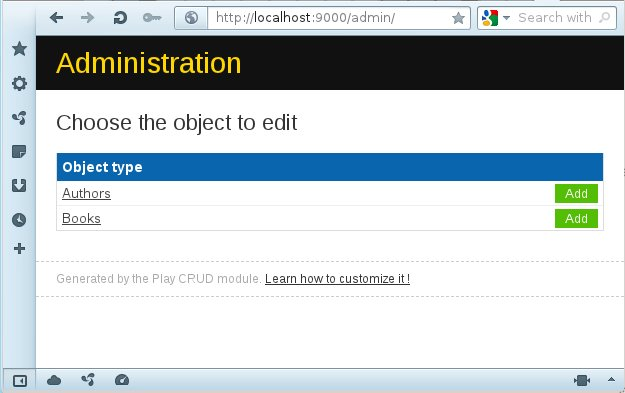
\includegraphics[scale=0.7]{images/crud1.jpeg}}
  \caption[CRUD interface for Play]{Figure depicts the CRUD interface which Play provides for simple model classes.}
  \label{fig:crud1}
\end{figure}
\begin{figure}[p]
  \centering
  \centerline{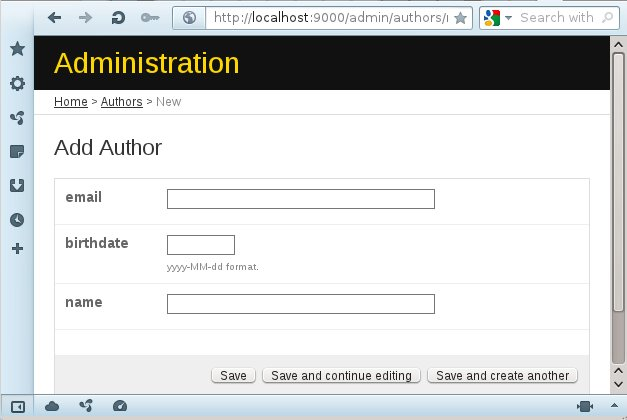
\includegraphics[scale=0.7]{images/crud2.jpeg}}
  \caption[CRUD interface for Play 2]{Figure depicts editing an Author object with the Play CRUD interface.}
  \label{fig:crud2}
\end{figure}

\subsection{Conclusion}
The tutorial has shown how the process of creating a code generator works. We start off by defining our DSML and a sample instance model and corresponding textual output.

Through the chapter we have seen the basic building blocks and features of a Xpand template, everything from defining the output to using extensions for abstracting away complex code. Lastly, we have seen how to generate a simple CRUD interface using Play.

The complete example project can be found at \url{http://dpf.hib.no/downloads/}, which includes Eclipse integration for the project.


% 
% create project in play!
% 
% 
% -constraints er ikkje handheva i generering
% - what to generate -> model classes
%   - input/output slik som definert i kap 3
% -create project
%   - bilete av vegvisar
%   - prosjektstruktur med generert workflow og template
% - defining a template 
%   - constructs som blir brukt
%   - extensions
% - project that uses the generator
% - utfordringar når ein ikkje har symbol, vanskelig å lage oversiktlege diagram.
% - debugging the workflow
% Things to add:
% \begin{itemize}
%     \item Introduction to Play Framework
%     \item How to it works
%     \item Describe process of creating generator from beginning to end
%     \item Illustration showing how the project interacts with *metamodel and *ui
%     \item Illustration showing typed template editor?
% \end{itemize}